\documentclass[aspectratio=169]{beamer}

% ---------- THEME & LOOK ----------
\usetheme{Madrid}
\usecolortheme{seahorse}
\usefonttheme{professionalfonts}
\setbeamertemplate{navigation symbols}{}
\setbeamercovered{transparent}
\setbeamertemplate{itemize items}[circle]
\setbeamertemplate{enumerate items}[default]
\setlength{\parskip}{0.25em}



% ---------- COLORS ----------
\usepackage{xcolor}
\definecolor{accent}{RGB}{0,92,184}   % deep academic blue
\setbeamercolor{structure}{fg=accent}
\setbeamercolor{title}{fg=white,bg=accent}
\setbeamercolor{frametitle}{fg=accent}
\setbeamercolor{block title}{bg=accent!10,fg=accent}
\setbeamercolor{block body}{bg=accent!3}


% ---------- PACKAGES ----------
\usepackage{booktabs}
\usepackage{graphicx}
\usepackage{array}
\usepackage{amsmath}
\usepackage{caption}
\usepackage{hyperref}
\hypersetup{colorlinks=true,linkcolor=accent,urlcolor=accent}

\newcommand{\placeholderbox}[2][0.8\linewidth]{%
  \begin{center}
    \fbox{\begin{minipage}[c][0.45\textheight][c]{#1}
      \centering \vspace{0.5em}
      \textbf{#2}\\[0.75em]
      \emph{Insert figure/diagram here later.}
    \end{minipage}}
  \end{center}
}

% ---------- TITLE ----------
\title{\textbf{Introduction to Labour Market Economics \vspace{.5cm}\\  }}
\subtitle{ {\large ECON 300 - Labour Economics}}
%\institute{UNBC}
\author{Muhebullah Karimzada}

\date{Winter 2026}



\begin{document}

\begin{frame}[plain]
  \titlepage
\end{frame}

% ============================================================
\begin{frame}{Learning Objectives}
\begin{itemize}
  \item Understand that earnings, hours, and hourly wages are unevenly distributed.
  \item Learn how supply and demand determine equilibrium wages and employment.
  \item Identify how laws and institutions affect labour market outcomes.
  \item Explore different data types (time-series, cross-section, panel).
  \item Understand econometric tools like regression analysis.
\end{itemize}
\end{frame}

% ============================================================
\begin{frame}{Main Questions}
\begin{itemize}
  \item Who are the main actors in the labour market?
  \item How do supply and demand interact?
  \item What types of policy questions does labour economics address?
  \item What makes the labour market different from other markets?
  \item What is the neoclassical model of labour markets?
\end{itemize}
\end{frame}

% ============================================================
\begin{frame}{Main Players and Roles: Individuals}
\begin{itemize}
  \item Decide when to enter or exit the labour force.
  \item Choose how much education and training to pursue.
  \item Determine hours of work, job type, and location.
  \item Evaluate wages, benefits, and work-life balance.
\end{itemize}
\textbf{Example:} Deciding between full-time work or continuing education involves weighing opportunity costs and future wages.
\end{frame}

% ============================================================
\begin{frame}{Main Players and Roles: Firms}
\begin{itemize}
  \item Determine how many workers to hire.
  \item Decide on wage and benefit levels.
  \item Adjust hours, layoffs, or outsourcing.
  \item Plan pensions and retirement policies.
\end{itemize}
\textbf{Example:} A retailer may hire extra workers during holidays when expected sales rise.
\end{frame}

% ============================================================
\begin{frame}{Factors Influencing Firm Decisions}
\begin{itemize}
  \item \textbf{Global Competition:} Free trade, deregulation, restructuring.
  \item \textbf{Legislative Environment:} Minimum wage, parental leave, safety standards.
  \item \textbf{Changing Workforce:} Demographics, diversity, aging.
\end{itemize}
\end{frame}

% ============================================================
\begin{frame}{Main Players and Roles: Government}
\begin{itemize}
  \item Balances worker protection and firm competitiveness.
  \item Provides EI, training, pensions, and insurance.
  \item Shapes collective bargaining laws and standards.
\end{itemize}
\end{frame}

% ============================================================
\begin{frame}{Labour Market Economics}
\textbf{Definition:} Labour economics studies how wages, employment, and unemployment are determined by the interaction of labour supply and demand.
\begin{block}{Key Idea}
The labour market links people’s time and skills with firms’ demand for productive inputs.
\end{block}
\end{frame}

% ============================================================
\begin{frame}{Dimensions of Labour Supply}
\begin{block}{Quantity Dimensions}
Population growth and participation rates.
\end{block}
\begin{block}{Quality Dimensions}
Education, health, and productivity.
\end{block}
\begin{block}{Income Maintenance Programs}
Welfare, disability, and employment insurance affect incentives to work.
\end{block}
\end{frame}

% ============================================================
\begin{frame}{Dimensions of Labour Demand}
\begin{itemize}
  \item Labour costs (wages, benefits, mandated costs).
  \item Demand for output (product demand drives labour demand).
  \item Globalization, free trade, and technological change.
\end{itemize}
\end{frame}

% ============================================================
\begin{frame}{Labour Market Outcomes}
\begin{itemize}
  \item Wages, employment, unemployment, and wage differentials.
  \item Influenced by laws, unions, and market structure.
\end{itemize}
\end{frame}

% ============================================================
\begin{frame}{Sources of Income for Canadians, 2017}
\begin{table}[h!]
\centering
\caption{Table 1.1: Sources of Income for Individual Canadians, 2017}
\small
\begin{tabular}{lccc}
\toprule
 & \textbf{Full Sample} & \textbf{Men} & \textbf{Women} \\
\midrule
Earnings & 41,348 & 50,824 & 31,910 \\
Investment income & 2,542 & 2,906 & 2,179 \\
Pension income & 1,262 & 1,484 & 1,040 \\
Other income & 952 & 971 & 933 \\
Gov. transfers & 3,728 & 2,495 & 4,955 \\
\midrule
Subtotal & 49,831 & 58,681 & 41,017 \\
Income taxes & 8,391 & 11,168 & 5,625 \\
After-tax total & 41,440 & 47,512 & 35,392 \\
Hours worked & 1,411 & 1,593 & 1,230 \\
Hourly wage & 29.77 & 32.57 & 26.67 \\
\bottomrule
\end{tabular}
\end{table}
\end{frame}

% ============================================================
% Figure Slides (placeholders)
% ============================================================

\begin{frame}{Figure 1.1: Distribution of Individual Labour Earnings (2017)}
\centering
\vspace{2em}
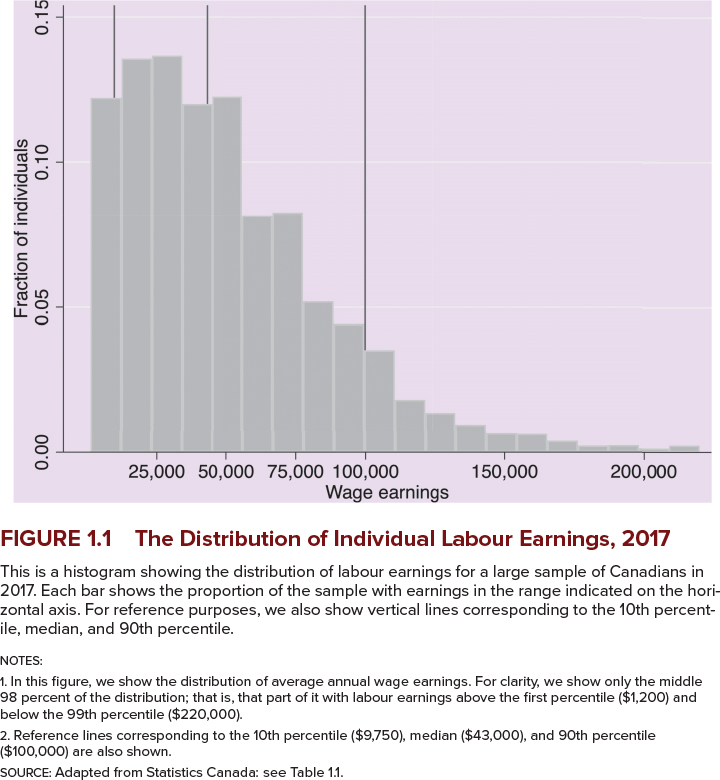
\includegraphics[width=0.57\linewidth]{ben54842_0101.jpg}
\captionof{figure}{Placeholder – Add the figure showing skewed earnings distribution later.}
\end{frame}

\begin{frame}{Figure 1.2: Distribution of Annual Hours Worked (2017)}
\centering
\vspace{2em}
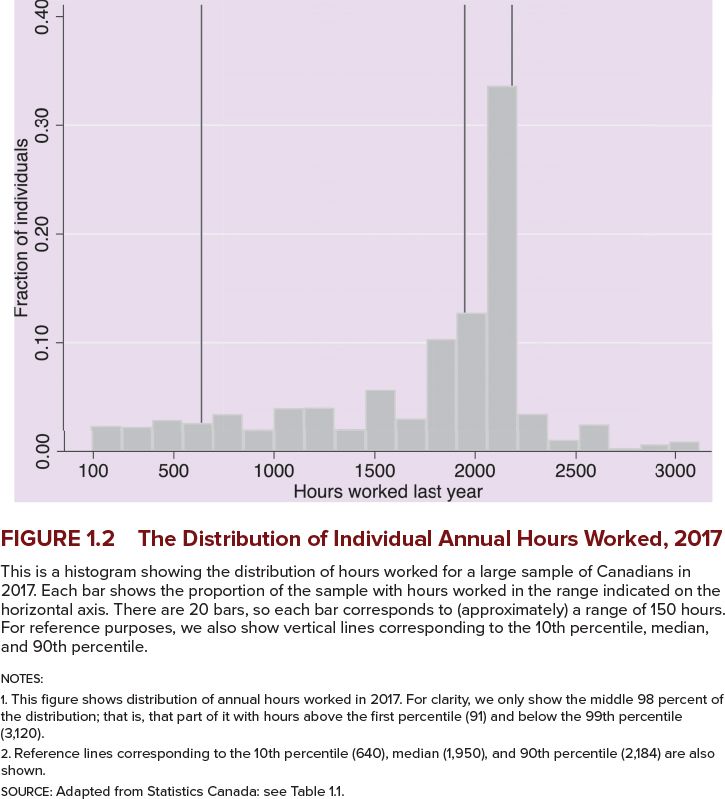
\includegraphics[width=0.57\linewidth]{ben54842_0102.jpg}
\captionof{figure}{Placeholder – Insert hours worked distribution diagram.}
\end{frame}

\begin{frame}{Figure 1.3: Distribution of Average Hourly Earnings (2017)}
\centering
\vspace{2em}
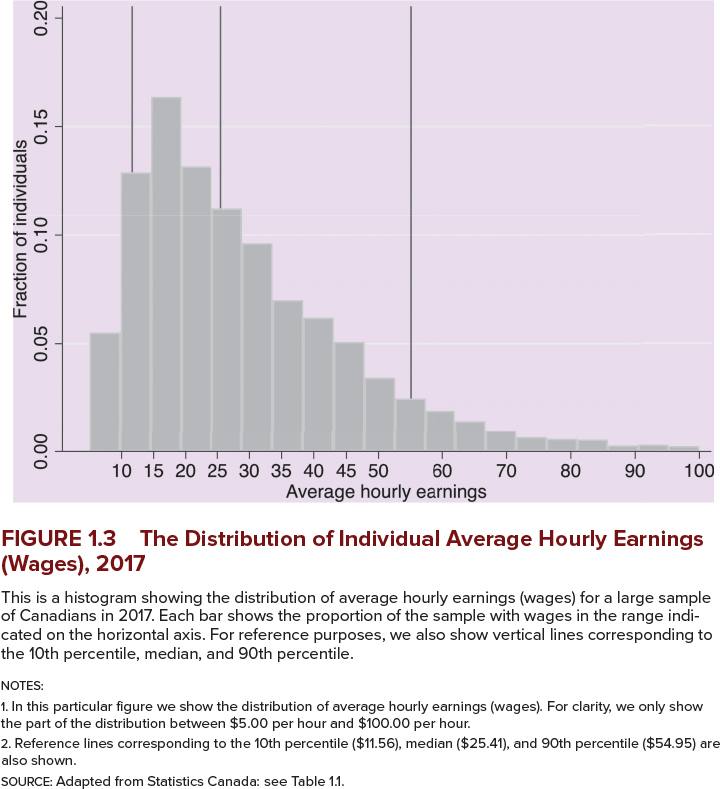
\includegraphics[width=0.55\linewidth]{ben54842_0103.jpg}
\captionof{figure}{Placeholder – Insert hourly earnings histogram.}
\end{frame}

% ============================================================
\begin{frame}{Neoclassical Model of Labour Supply and Demand}
\begin{itemize}
  \item Workers supply labour to maximize utility.
  \item Firms demand labour to maximize profit.
  \item Market equilibrium determines wage and employment.
\end{itemize}
\end{frame}

\begin{frame}{Figure 1.4: Wages and Employment in a Competitive Market}
\centering
\vspace{2em}
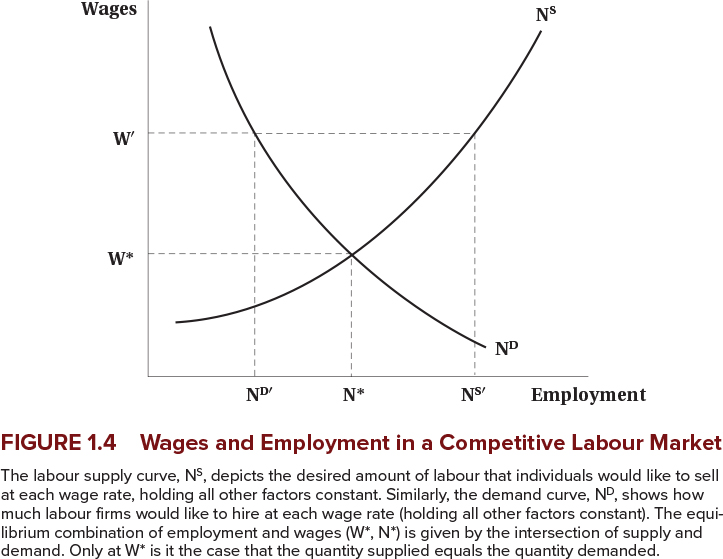
\includegraphics[width=0.7\linewidth]{ben54842_0104.jpg}
\captionof{figure}{Placeholder – Insert labour supply and demand equilibrium graph.}
\end{frame}

\begin{frame}{Figure 1.5: Equilibrium Wages Across Two Sectors}
\centering
\vspace{2em}
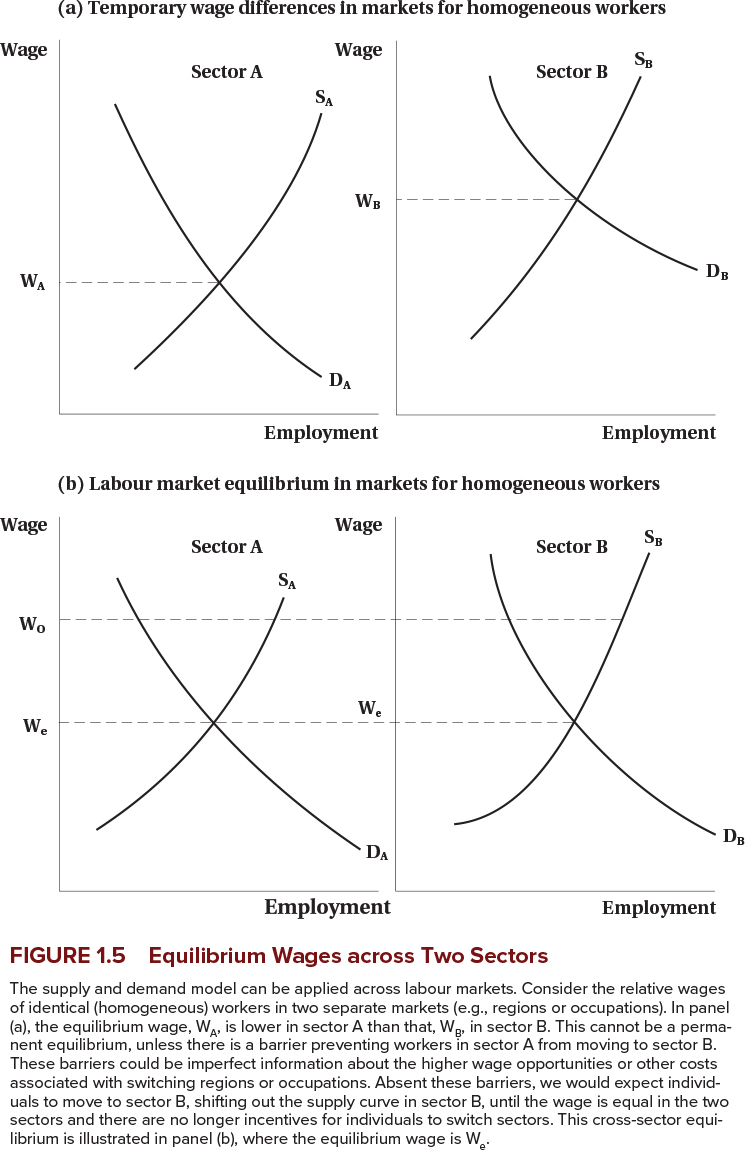
\includegraphics[width=0.34\linewidth]{ben54842_0105.jpg}
\captionof{figure}{Placeholder – Add diagram comparing sectoral equilibrium wages.}
\end{frame}

% ============================================================
\begin{frame}{Current Policy Issues}
\begin{itemize}
  \item \textbf{Labour Supply:} Impact of EI, welfare, and childcare.
  \item \textbf{Labour Demand:} Effects of trade, outsourcing, and regulation.
  \item \textbf{Wage Structures:} Gender gaps, benefits, and equity.
  \item \textbf{Unemployment:} Youth and cyclical unemployment trends.
\end{itemize}
\end{frame}

% ============================================================
\begin{frame}{COVID-19 and the Labour Market}
\begin{itemize}
  \item Widespread layoffs and remote work adjustments.
  \item Disproportionate impact on low-income earners.
  \item Parents reduced hours due to childcare closures.
\end{itemize}
\end{frame}

\begin{frame}{Figure 1.6: COVID-19 Employment Losses Across Earning Quartiles}
\centering
\vspace{2em}
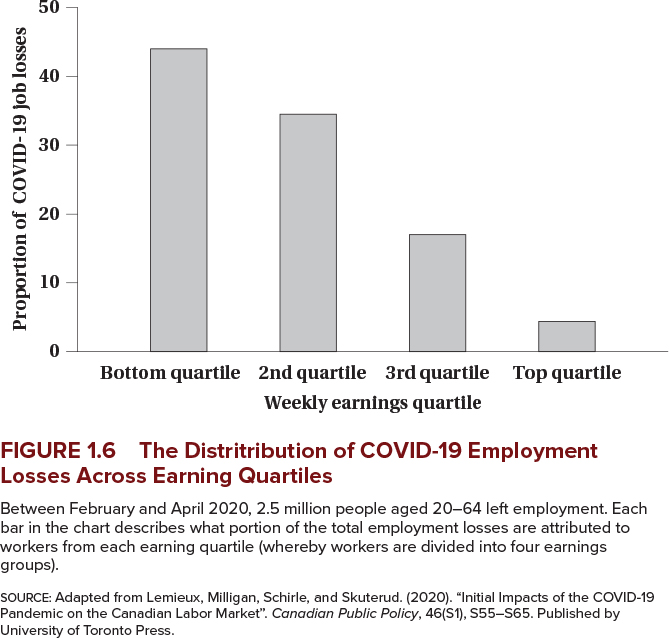
\includegraphics[width=0.6\linewidth]{ben54842_0106.jpg}
\captionof{figure}{Placeholder – Insert COVID-19 employment losses bar chart.}
\end{frame}

% ============================================================
\begin{frame}{Labour Market vs. Other Markets}
\begin{itemize}
  \item Actors pursue diverse goals beyond profit.
  \item Influenced by legal, institutional, and social factors.
  \item Wages serve as price, signal, and incentive simultaneously.
\end{itemize}
\end{frame}

% ============================================================
\begin{frame}{Summary}
\begin{itemize}
  \item Main actors: individuals, firms, and government.
  \item Outcomes: wages, employment, hours.
  \item Neoclassical model as key analytical tool.
  \item Institutional and policy factors modify market outcomes.
\end{itemize}
\end{frame}

% ============================================================
\begin{frame}{Appendix 1A: Regression Analysis and Research Design}
\begin{itemize}
  \item Data types: time-series, cross-section, and panel.
  \item Empirical tools link labour outcomes with determinants.
  \item Example: NHL player salaries and performance.
\end{itemize}
\end{frame}

\begin{frame}{Figure 1.A1: Supply and Demand – “Star” vs. “Grinder” Players}
\centering
\vspace{2em}
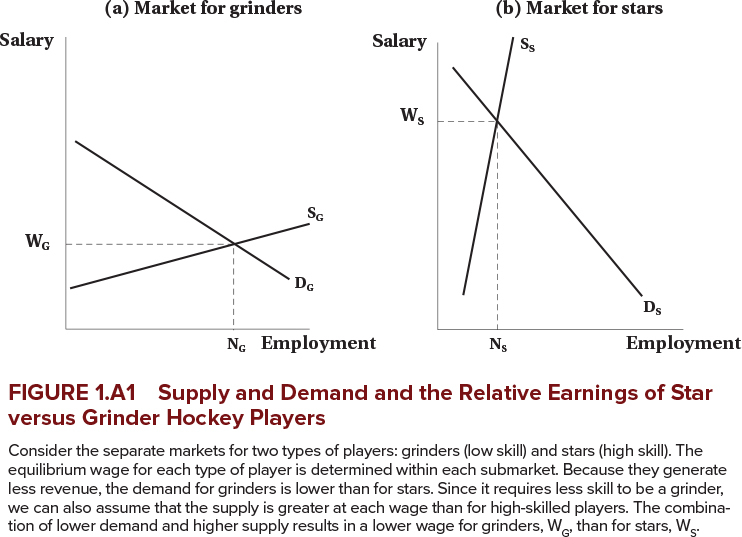
\includegraphics[width=0.75\linewidth]{ben54842_01a1.jpg}
\captionof{figure}{Placeholder – Insert figure showing relative earnings between star and grinder players.}
\end{frame}

\begin{frame}{Figure 1.A2: NHL Player Salaries by Goals Scored (2018–19)}
\centering
\vspace{2em}
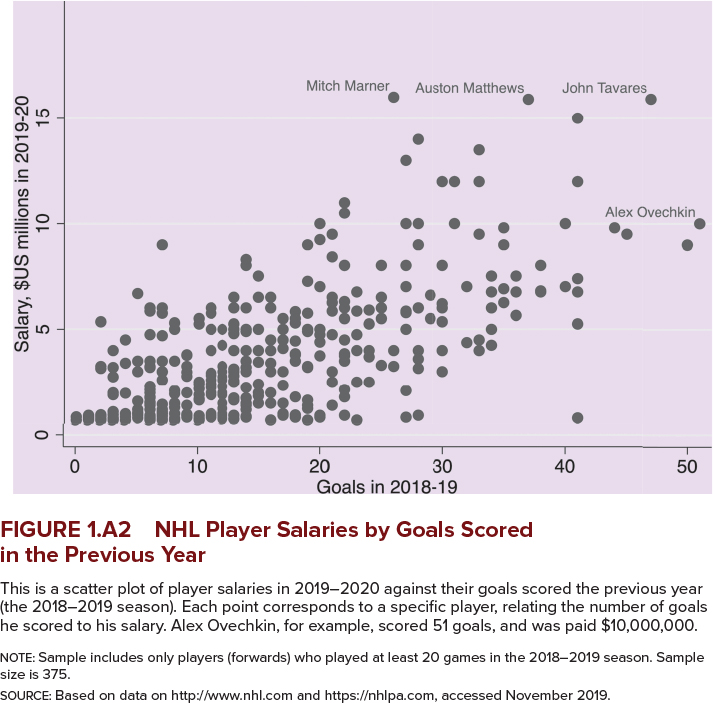
\includegraphics[width=0.55\linewidth]{ben54842_01a2.jpg}
\captionof{figure}{Placeholder – Insert scatterplot showing goals vs. salary.}
\end{frame}

\begin{frame}{Figure 1.A3: Log Salary and Goals with Regression Line (2018–19)}
\centering
\vspace{2em}
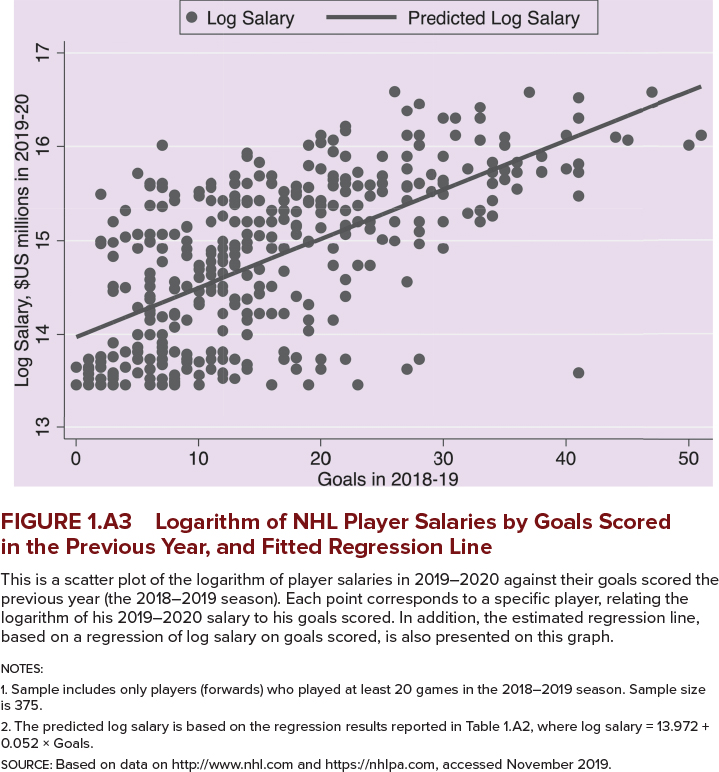
\includegraphics[width=0.57\linewidth]{ben54842_01a3.jpg}
\captionof{figure}{Placeholder – Insert fitted regression line on log-salary plot.}
\end{frame}

% ============================================================
\begin{frame}{Tabulation of NHL Player Salaries by Goals Scored}
\begin{table}[h!]
\centering
\caption{Table 1.A1: NHL Player Salaries by Goals Scored, 2018–19}
\small
\begin{tabular}{lccc}
\toprule
Goals & Sample Size & Salary (millions) & $\ln$(Salary) \\
\midrule
0–9 & 121 & 1.93 & 14.20 \\
10–19 & 133 & 3.13 & 14.73 \\
20–29 & 76 & 5.53 & 15.32 \\
30–39 & 32 & 7.51 & 15.76 \\
40–49 & 11 & 9.03 & 15.82 \\
50+ & 2 & 9.50 & 16.07 \\
\bottomrule
\end{tabular}
\end{table}
\end{frame}

\begin{frame}{Estimated Effects of Performance on Salary (OLS, 2019–20)}
\begin{table}[h!]
\centering
\caption{Table 1.A2: OLS Estimates of Player Salary Determinants}
\scriptsize
\begin{tabular}{lcccccc}
\toprule
 & (1) & (2) & (3) & (4) & (5) & (6) \\
\midrule
Intercept & 685,592 & 247,395 & 197,563 & 13.972 & 13.867 & 13.859 \\
Goals & 195,498 & 88,605 & 90,550 & 0.052 & 0.027 & 0.027 \\
Assists &  & 98,218 & 98,902 &  & 0.024 & 0.024 \\
Plus/Minus &  &  & -8,156 &  &  & -0.001 \\
$R^2$ & 0.44 & 0.54 & 0.54 & 0.39 & 0.47 & 0.47 \\
\bottomrule
\end{tabular}
\end{table}
\end{frame}

% ============================================================
\begin{frame}{Appendix 1B: Research Designs in Labour Economics}
\begin{itemize}
  \item Experimental: Random assignment (treatment vs. control).
  \item Non-experimental: Regression, DiD, natural experiments.
  \item Purpose: Estimate counterfactuals—what would happen without policy change.
\end{itemize}
\end{frame}

\begin{frame}
\centering
\Huge{\textbf{Thank You!}} \\

\end{frame}

\end{document}